\documentclass{article}

\usepackage{titlesec}
\usepackage{amsmath}
\usepackage{amsfonts}
\usepackage{graphicx}
\usepackage{float}
\title{Numerical Methods for Ordinary Differential Equations}
\author{Murray Heymann \\
	Technische Universit{\"a}t Kaiserslautern \\
	413121}
\date{\today}


\titleformat{\section}{\normalfont \LARGE \bfseries}
{Problem\ Sheet\ \thesection}{2.3ex plus .2ex}{}
\titleformat{\subsection}{\normalfont \Large \bfseries}
{Question\ \thesubsection}{2.3ex plus .2ex}{}
\titlespacing{\subsubsection}{2em}{*1}{*1}

\begin{document}
\maketitle


\setcounter{section}{1}
\section{}
\subsection{}
Since these implementation has significantly smaller error, we use a relatively
large step value in the following graphs.
\begin{figure}[H]
	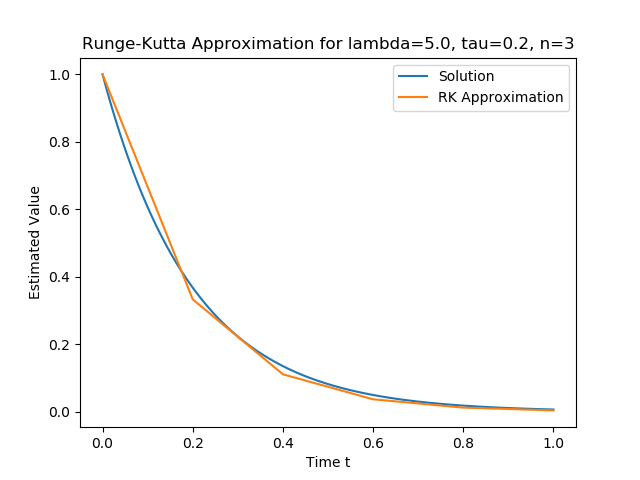
\includegraphics[scale=0.6]{RK3_02_5}
\end{figure}
\begin{figure}[H]
	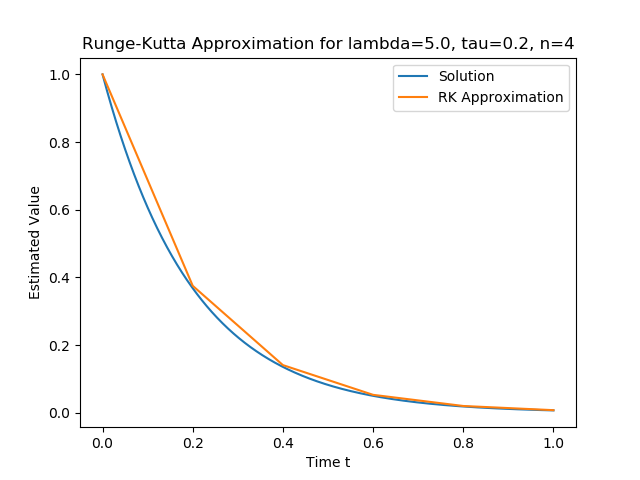
\includegraphics[scale=0.6]{RK4_02_5}
\end{figure}

To confirm the degree numerically, we have to look at the gradient of the
log-log graphs.

\begin{figure}[H]
	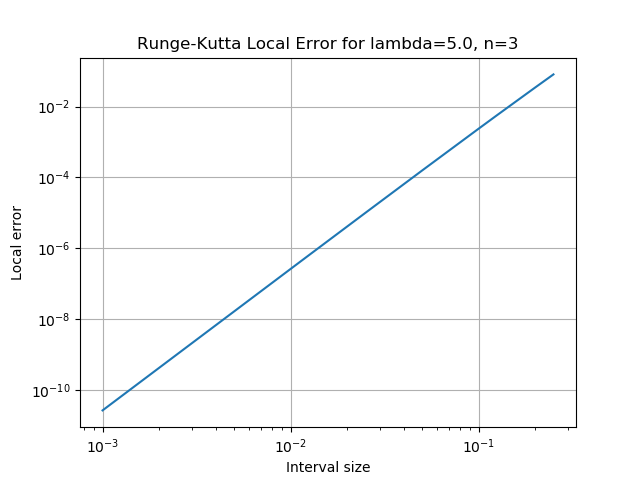
\includegraphics[scale=0.6]{RK3_5_loglog}
\end{figure}
The Runge-Kutta method with $3$ stages yields a log-log line graph with a
gradient of $4$.  This is in keeping with an approximation of order $3$.
\begin{figure}[H]
	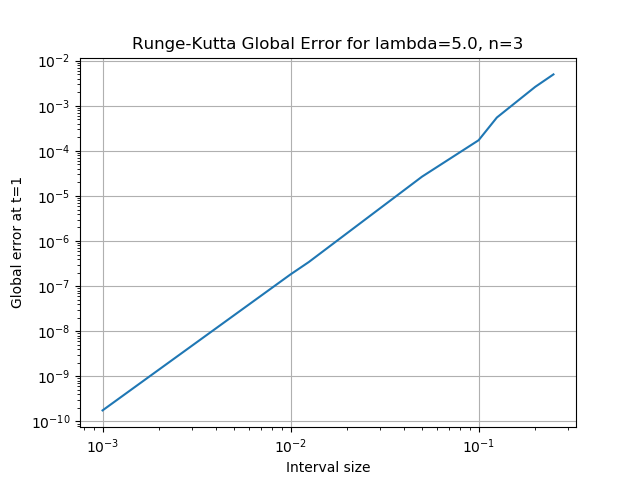
\includegraphics[scale=0.6]{RK3_5_loglog_global}
\end{figure}
The log-log graph for the global error of the Runge-Kutta method with $3$
stages is a line graph with a gradient of $3$, confirming that the method is of
order $3$. Note that for interval sizes of greater than $0.1$, the graph becomes
irregular.

\begin{figure}[H]
	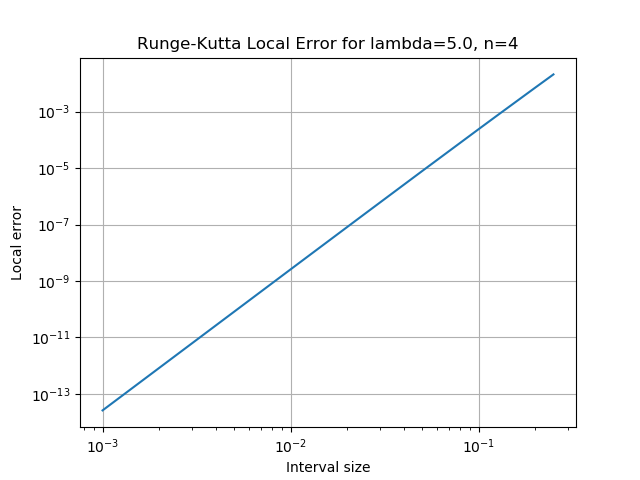
\includegraphics[scale=0.6]{RK4_5_loglog}
\end{figure}
The Runge-Kutta method with $4$ stages yields a log-log line graph with a
gradient of $5$.  This is in keeping with an approximation of order 4.
\begin{figure}[H]
	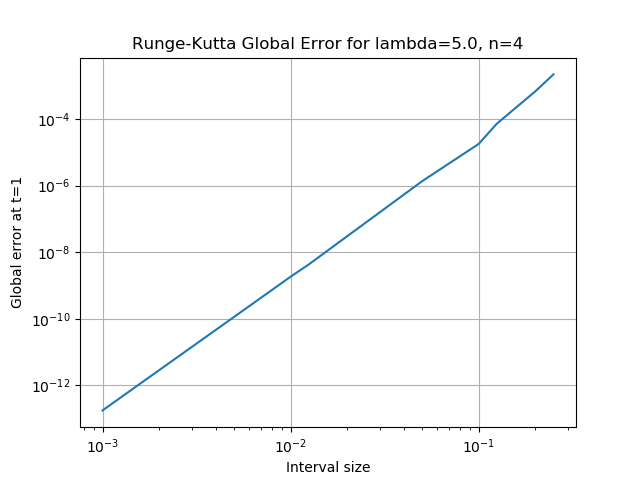
\includegraphics[scale=0.6]{RK4_5_loglog_global}
\end{figure}
The log-log graph for the global error of the Runge-Kutta method with $4$
stages is a line graph with a gradient of $4$, confirming that the method is of
order $4$. Note that for interval sizes of greater than $0.1$, the graph becomes
irregular.


\subsection{}
\begin{itemize}
	\item[(a),(b)]
		As adaptive Runge-Kutta method described in the notes required
		two embedded RK-approximations, the two approximations from
		Exercise $1$ aren't ideal candidates for an adaptive method.
		Nevertheless, an adaptive method could still be made, although it
		is more computationally intensive than the embedded case might
		have been.

		In each step, the step size is initially set to a maximum value.
		\[
			\tau_{i+1} := \tau_{\text{max}}
		\]
		Using this step size, the next estimate is calculated using the
		four step ($\mathbf{x}_{i+1}^{\Delta 4}$) and the three step
		($\mathbf{x}_{i+1}^{\Delta 3}$) RK-method. The results are then
		subtracted to get an error value.
		\[
			\epsilon_{i + 1} := |\mathbf{x}_{i+1}^{\Delta 4} -
			\mathbf{x}_{i+1}^{\Delta 3}|
		\]
		If the error value is more than the acceptable tolerance, the
		step size is updated
		\[
			\tau_{i+1}:= \tau_{j+1} \sqrt[p+1]{\frac{\rho.
			\text{tol}}{\epsilon_{i + 1}}}
		\]
		The error value is then calculated again.  This is repeated
		until the error is within the required tolerance, in which case
		the estimate of the $4$ step RK method is recorded.

		We know that $\mathbf{x}_{i+1}^{\Delta 3}$ and
		$\mathbf{x}_{i+1}^{\Delta 4}$ are satisfy
		\begin{align*}
			\mathbf{x}_{i}^{\Delta 4} = \mathbf{x}_{i} +
			\mathcal{O}(\tau^5) \\
			\mathbf{x}_{i}^{\Delta 3} = \mathbf{x}_{i} +
			\mathcal{O}(\tau^4)
		\end{align*}
		so their difference is given by
		\begin{align*}
			\mathbf{x}_{i}^{\Delta 4} - \mathbf{x}_{i}^{\Delta 3} =
			C_i \tau^4 + \mathcal{O}(\tau^5)
		\end{align*}
		Therefore this can be made arbitrarily small, by decreasing the
		size of $\tau$.

		As only a finite number of steps $n$ are followed, and each error
		made by each step is bounded by $K_i \tau_i^5$ (the local error of
		the four step RK approximation), the global error must be
		bounded by
		\[
			\epsilon_g \leq n \max(K_i) \max(\tau_i)^5
		\]
		\begin{figure}[H]
			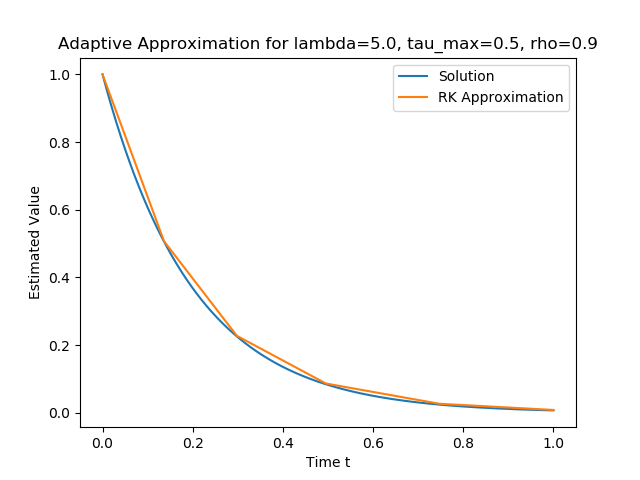
\includegraphics[scale=0.6]{adaptive}
		\end{figure}

	\item[(c)]
		As the values for the solutions tend to get very large in
		absolute value, this report restricted values for $\mu$ to under
		$8$. For some small values of $\mu$, the entire phase graph was
		approximated with the adaptive method.
		\begin{figure}[H]
			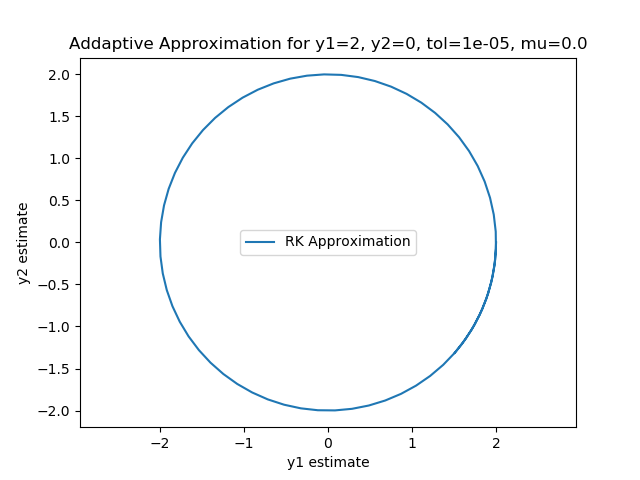
\includegraphics[scale=0.6]{adapt_vdp0}
		\end{figure}
		\begin{figure}[H]
			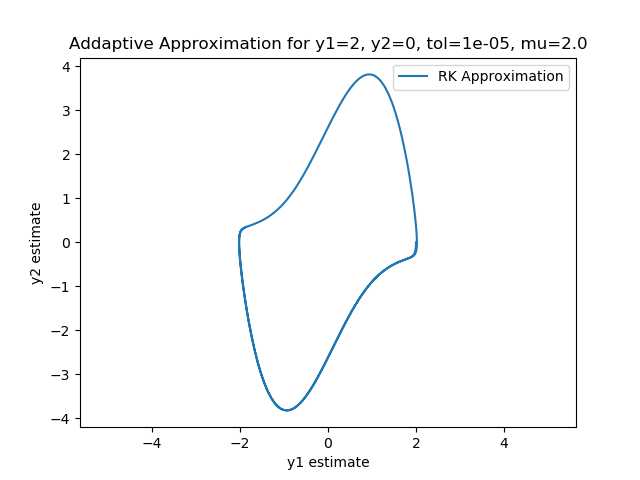
\includegraphics[scale=0.6]{adapt_vdp2}
		\end{figure}
		\begin{figure}[H]
			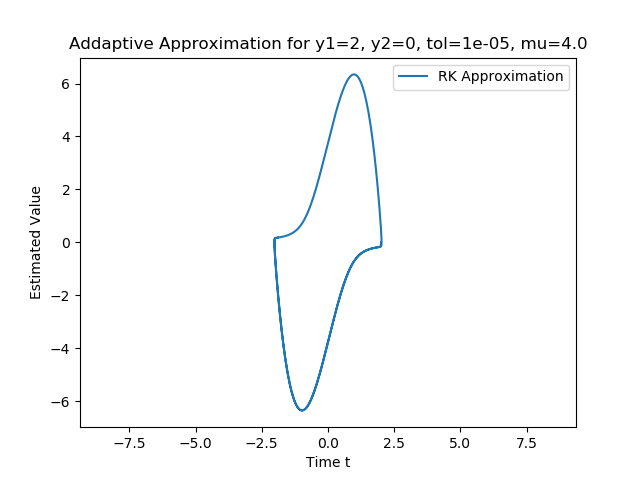
\includegraphics[scale=0.6]{adapt_vdp4}
		\end{figure}
		\begin{figure}[H]
			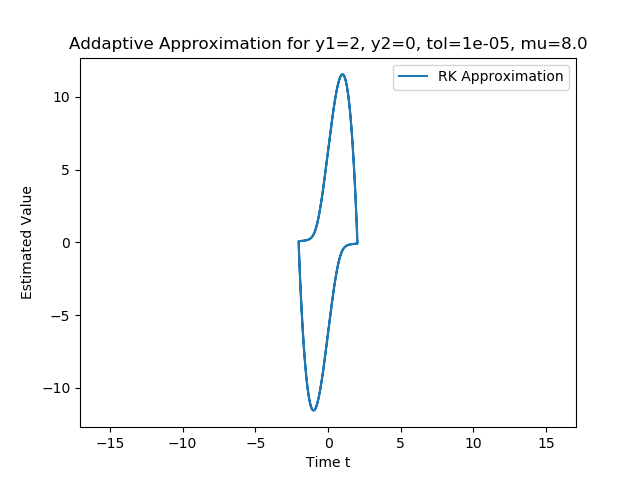
\includegraphics[scale=0.6]{adapt_vdp8}
		\end{figure}

		For a fixed value of $\mu=2$, various starting values were used,
		as graphed below:
		\begin{figure}[H]
			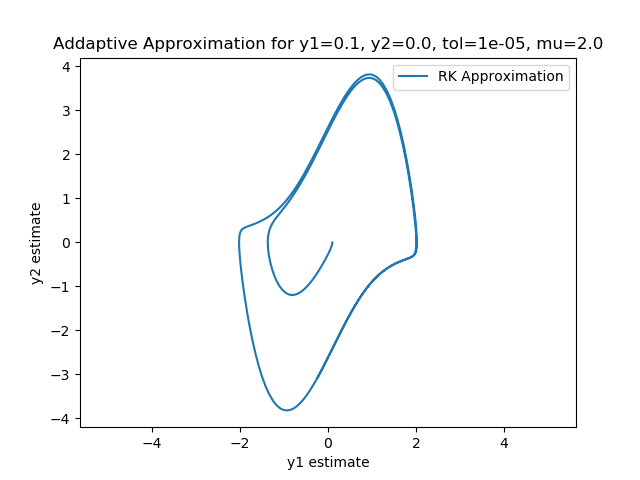
\includegraphics[scale=0.6]{start_2_01_0}
		\end{figure}
		\begin{figure}[H]
			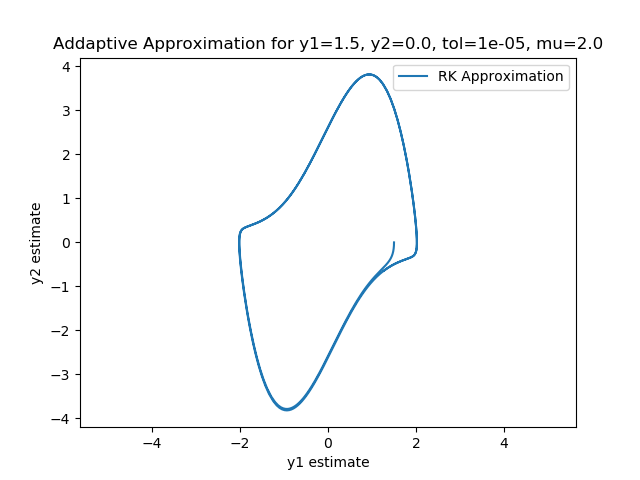
\includegraphics[scale=0.6]{start_2_15_0}
		\end{figure}
		\begin{figure}[H]
			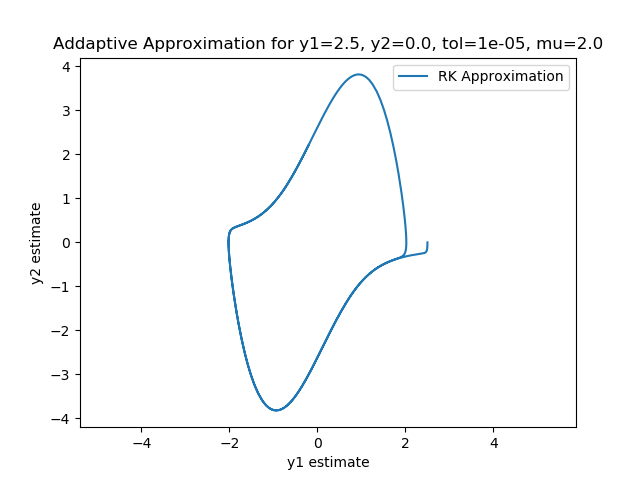
\includegraphics[scale=0.6]{start_2_25_0}
		\end{figure}
		\begin{figure}[H]
			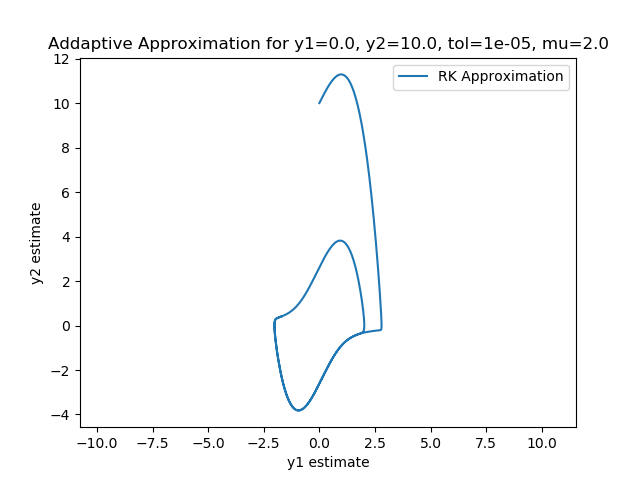
\includegraphics[scale=0.6]{start_2_0_10}
		\end{figure}
		Interestingly, the solution seems to quickly approach the $(2,
		0)$ solution, rather than make a larger figure, as would be the
		cased for an undamped oscillator.

		The variation in the time step sizes is visualized below:
		\begin{figure}[H]
			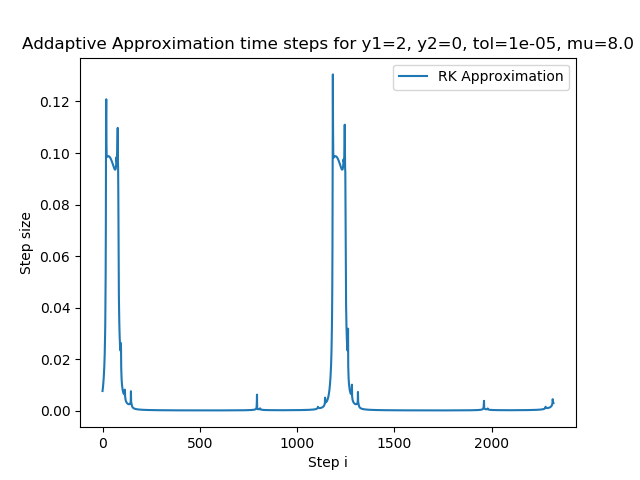
\includegraphics[scale=0.6]{adapt_times}
		\end{figure}

		Finally, the number of time-steps taken for various values of
		$\mu$ is given in the following graph:
		\begin{figure}[H]
			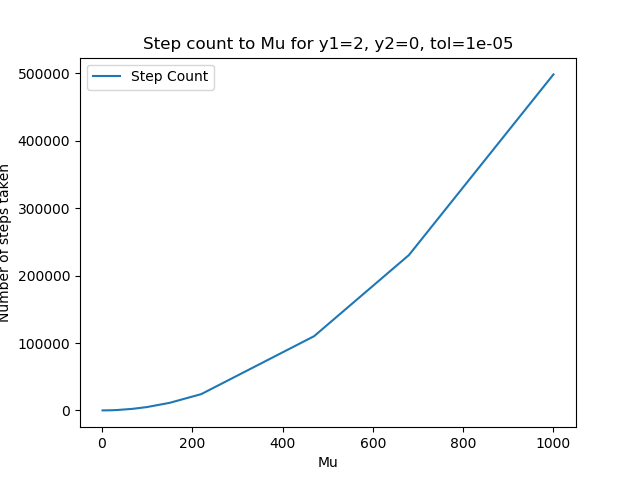
\includegraphics[scale=0.6]{Mu_to_steps}
		\end{figure}

		A log-log graph would not be appropriate here, as this is not a
		reflection of the quality of the estimation:  different values
		of $\mu$ yields fundamentally different graphs, which may or may
		not require more steps to estimate. 
\end{itemize}
\end{document}
